\chapter{Проведение экспериментов} \label{cha:experiments}
% QUESTION НУЖНО ЛИ ПЕРЕРИСОВЫВАТЬ КАРТИНКИ? А ССЫЛКИ НА КАРТИНКИ?

\section{Используемые инструменты}
% QUESTION: нужно это вообще?
Разработка велась на языке программирования \textit{Python 3.8}.
% QUESTION: правильно сослался?
Реализация нейронных сетей и оценка качества выполнены с помощью библиотек \textit{PyTorch} \cite{pytorch_lib}, \textit{transformers} и \textit{evaluate} от проекта \textit{HuggingFace} \cite{huggingface_transformers}.
Предобученные модели получены из \textit{HuggingFaceHub}, открытого репозиторя моделей и наборов данных.
Обучение выполнялось на видеокарте Nvidia T4.

\section{Метрики качества}
% QUESTION: тут цитаты нужно сделать? а что конкретно за веса, что взяты из хаггингфейса нужно сказать? если да, то как? а на берт нужно сослаться?

Для оценки качества алгоритма будут использоваться следующие метрики:
\begin{itemize}
    \item SacreBLEU \cite{sacrebleu};
    \item METEOR \cite{meteor};
    \item 
    Style Score -- дообученный с помощью параметро-эффективного метода LoRA \cite{lora} на собранном наборе данных классификатор стиля.
    В качестве изначальных весов взят \texttt{xlm-roberta-base}. Качество классификатора:
    \texttt{Accuracy}: 86\%,
    \texttt{F-1}: 86\%,
    \texttt{Precision}: 91\%,
    \texttt{Recall}: 83\%;
    \item 
    Semantic Score -- дообученный с помощью параметро-эффективного метода LoRA \cite{lora} на собранном наборе данных классификатор семантики, определяющий как сильно сохраняют два предложения одно и то же содержание.
    В качестве изначальных весов взят \texttt{cointegrated/rubert-tiny2}. Качество классификатора: 
    \texttt{Accuracy}: 85\%,
    \texttt{F-1}: 86\%,
    \texttt{Precision}: 91\%,
    \texttt{Recall}: 82\%.
\end{itemize}

\section{Обучение без учителя: Denoising Auto-Encoder}
% TODO подводку побольше
% QUESTION Этого одного цитирования достаточно на всё?
Генерация с помощью управления атрибутами с использованием архитектуры denoising auto-encoder \cite{lample2018unsupervised, lample2018phrasebased, subramanian2019multipleattribute} является распространённым решением в ситуации отсутствия параллельных данных.
% Естественным решением в ситуации отсутствия параллельных данных является unsupervised подход, который представлен denoising auto-encoder’ом \cite{lample2018unsupervised, lample2018phrasebased, subramanian2019multipleattribute}.

% Основная идея и принципы
% \subsection{Принципы}
% Задача изменения формальности текста является плохо сформулированной задачей, потому что потенциально существует множество способов перефразировать исходное предложение, особенно в неформальный стиль. 
% Тем не менее за последние годы был достигнут впечатляющий прогресс в достижении этой цели и были выделены основные принципы обучения без учителя, как для задачи переноса стиля текста, так и для задачи машинного перевода.

В данном подходе были выработаны три принципа для решения задачи.
Визуализация этих принципов представлена на рисунке \ref{fig:lample_principles}.
На изображении под пунктом A показаны исходные данные: два набора данных, каждый со своим стилем (разные цвета и точки соответствуют предложениям с соответствующим стилем).
Под пунктом Б представлен первый принцип: инициализация. Делается так, чтобы оба распределения примерно совпадали, например, с помощью дословного перевода с использованием словаря.
В пункте В проиллюстрирован второй принцип: языковое моделирование. Языковая модель обучается независимо для каждого стиля для определения структуры данных (изображено в виде непрерывной кривой); она действует как основанная на данных система для устранения шума / исправления предложений (проиллюстрировано пружиной, втягивающей предложение за пределы многообразия обратно).
И, наконец, под пунктом Г изображен третий принцип: обратный перевод (см. \ref{cha:analysis:subsection:backtranslation}).
Начиная с наблюдаемого исходного предложения (заполненный красный круг), используется текущая модель для парафраза (пунктирная стрелка), что приводит к потенциально неправильному переносу стиля (синий крестик рядом с пустым кругом).
Начиная с этого (обратного) перевода, используется модель для переноса стиля в обратную сторону (непрерывная стрелка) для восстановления предложения в оригинальном стиле.
Несоответствие между восстановлением и исходным предложением является сигналом ошибки для обучения параметрам модели.
    Та же процедура применяется в обратном направлении.
\begin{figure}[ht]
  \centering
  \frame{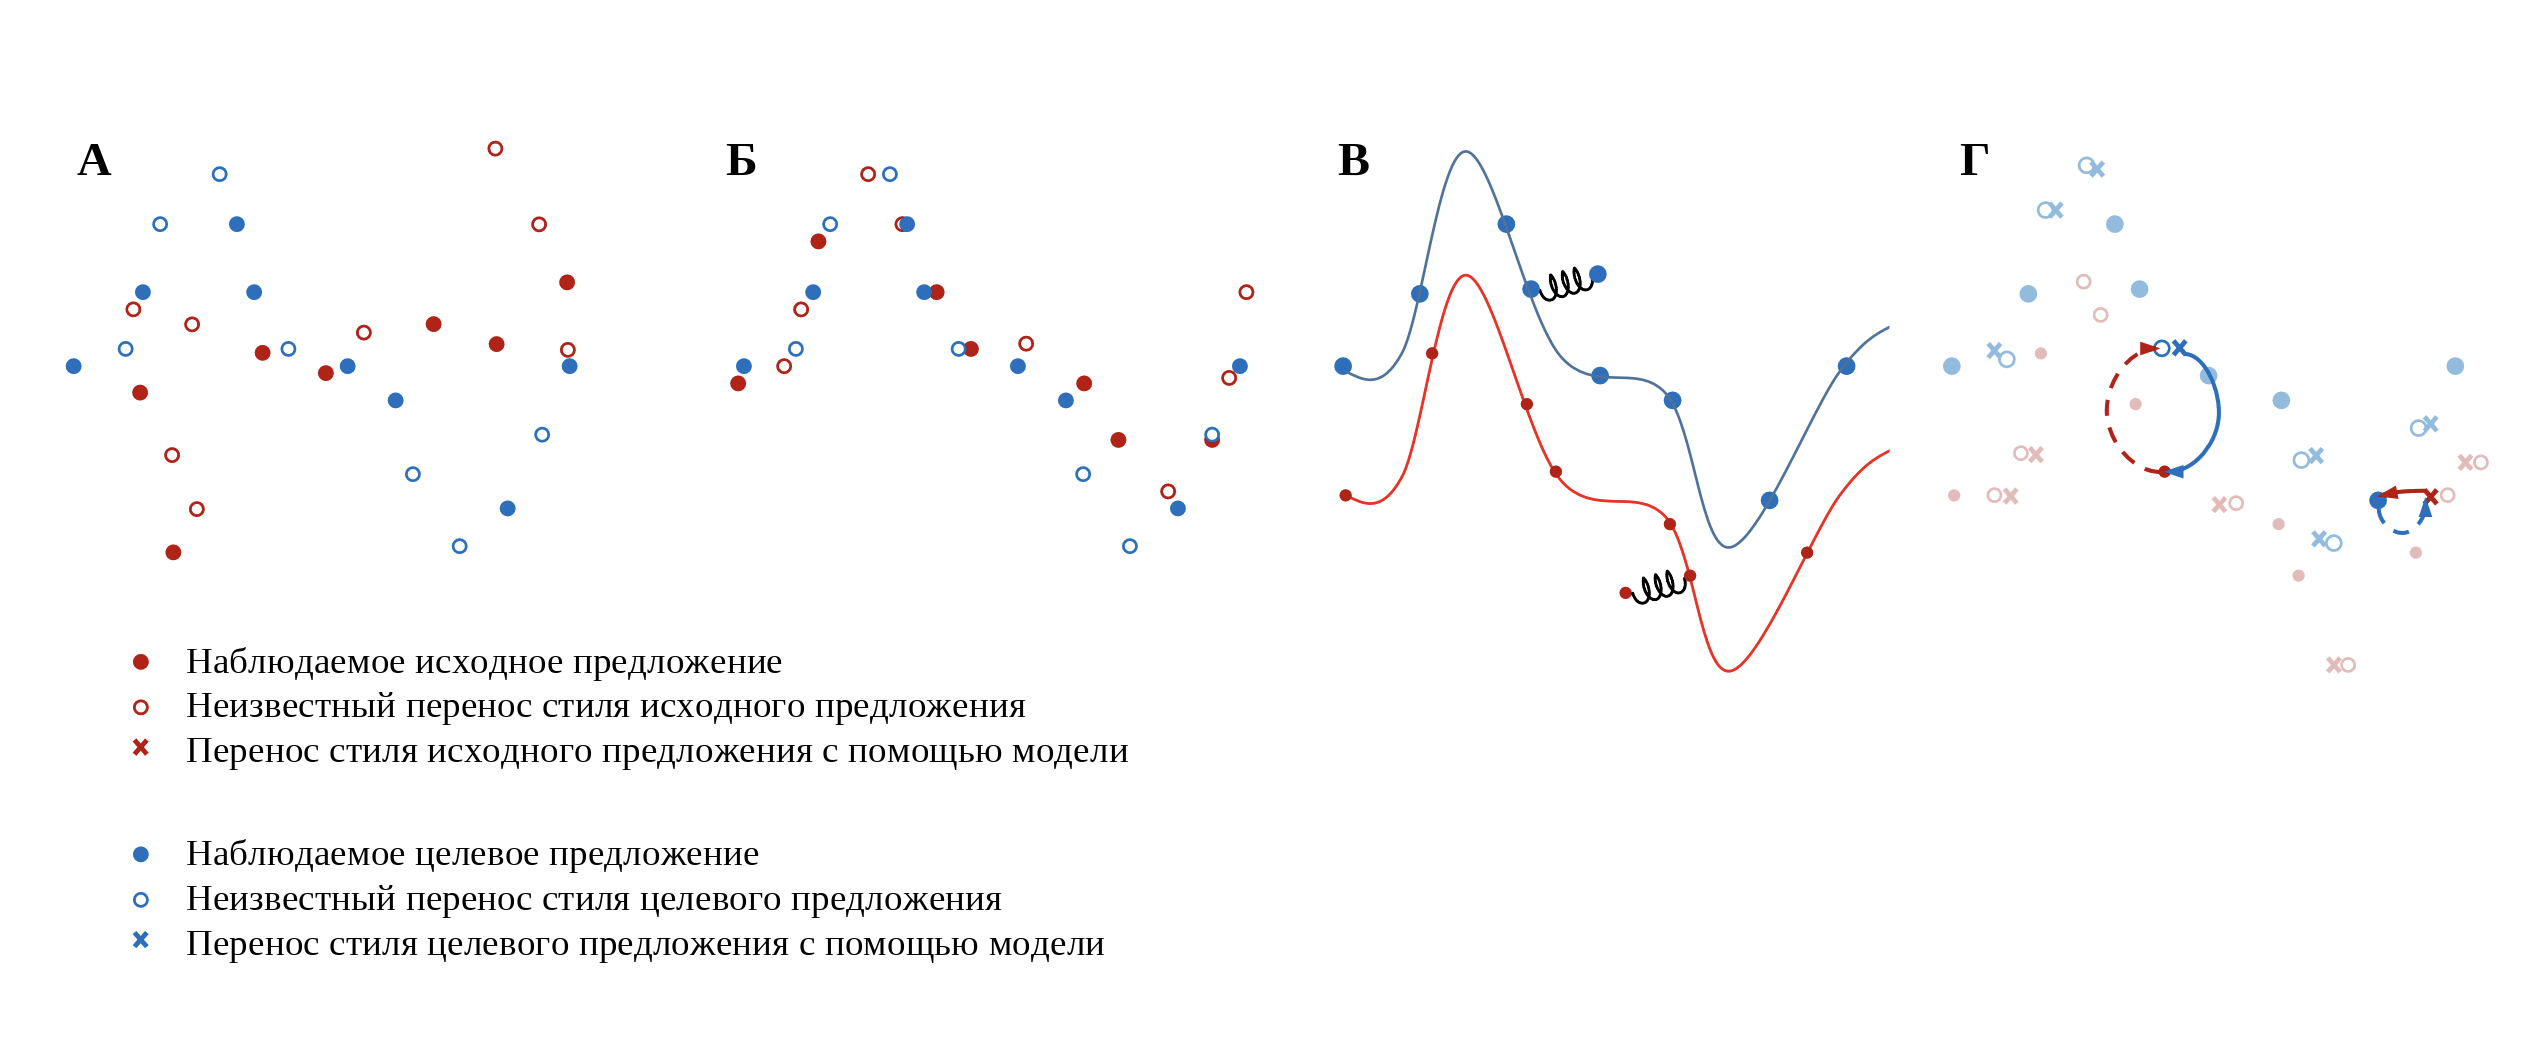
\includegraphics[width=\textwidth]{figures/lample_principles.png}}
  \caption{Принципы алгоритмов "без учителя" для задачи переноса стиля текста}
  \label{fig:lample_principles}
\end{figure}

% Архитектура (в разрезе принципов)
% \subsection{Архитектура модели}
% TODO: overview?
% QUESTION: алгоритм может в виде листинга представить??
% QUESTION: обозначиМ можно? можно в первом лице?
% Листинг алгоритма приведён на рисунке \ref{fig:lample_algorithm}.
% \begin{figure}[ht]
%   \centering
%   \frame{\includegraphics[width=\textwidth]{figures/lample_algorithm.png}}
%   \caption{Алгоритм обучения без учителя для переноса стиля текста}
%   \label{fig:lample_algorithm}
% \end{figure}

% \begin{figure}[ht]
%   \centering
%   \frame{\includegraphics[width=1.0\textwidth]{figures/analysis_lample.png}}
%   \caption{Генерация с помощью управления атрибутами с back-translation}
%   \label{fig:analysis_lample}
% \end{figure}

На этапе инициализации, вместо рассмотрения отдельных слов в предложении, используются byte-pair encoding токены (BPE-токены) \cite{bpe_tokens_article}.
Подобная токенизация даёт два больших преимущества: уменьшает размер словаря и избавляет от присутствия неизвестных UNK-токенов в перефразированном предложении.
BPE-токены обучаются на совместном наборе данных обоих стилей, так как язык одинаковый и большая часть этих токенов будет совпадать. Помимо прочего, в таком случае отпадает необходимость получать словарь между словами разного стиля.
Затем, обучаются word2vec эмбеддинги токенов \cite{mikolov2013distributed}, который затем будут использованы в языковой модели.

% Языковая модель состоит из 
Этап языкового моделирования представлен автокодировщиком с шумоподавлением (denoising autoencoder, DAE) \cite{dae_article, lample2018phrasebased}.
Архитектурой автокодировщика является transformer \cite{attention_is_all_you_need}.
Без каких-либо ограничений обычный автокодировщик очень быстро учится просто копировать каждое вводимое слово одно за другим.
Такая модель также идеально копировала бы последовательности случайных слов, предполагая, что модель не выучивает какую-либо полезную структуру в данных.
Чтобы решить эту проблему, во входные предложения добавляется шум \cite{hill2016learning} и применяется стратегия подавления шума, получая Denoising Autoencoder -- автокодировщик с шумоподавлением \cite{dae_article}.
Общая схема представлена на рисунке \ref{fig:lample_dae}, а функция потерь задаётся как:
$$
\mathcal{L}^{lm} = 
\mathbb{E}_{x \sim \mathcal{S}} [-\log P_{s \rightarrow s}(x|C(x))] +
\mathbb{E}_{y \sim \mathcal{T}} [-\log P_{t \rightarrow t}(y|C(y))]
$$

где $C$ - функция зашумления, которая удаляет или меняет местами некоторые слова \cite{lample2018unsupervised}, а $P_{s \rightarrow s}$ и $P_{t \rightarrow t}$ - композиции энкодера и декодера, оперирующие в исходном или целевом пространстве соответственно.

% QUESTION рассказать подробнее про функцию зашумления?

\begin{figure}[ht]
  \centering
  \frame{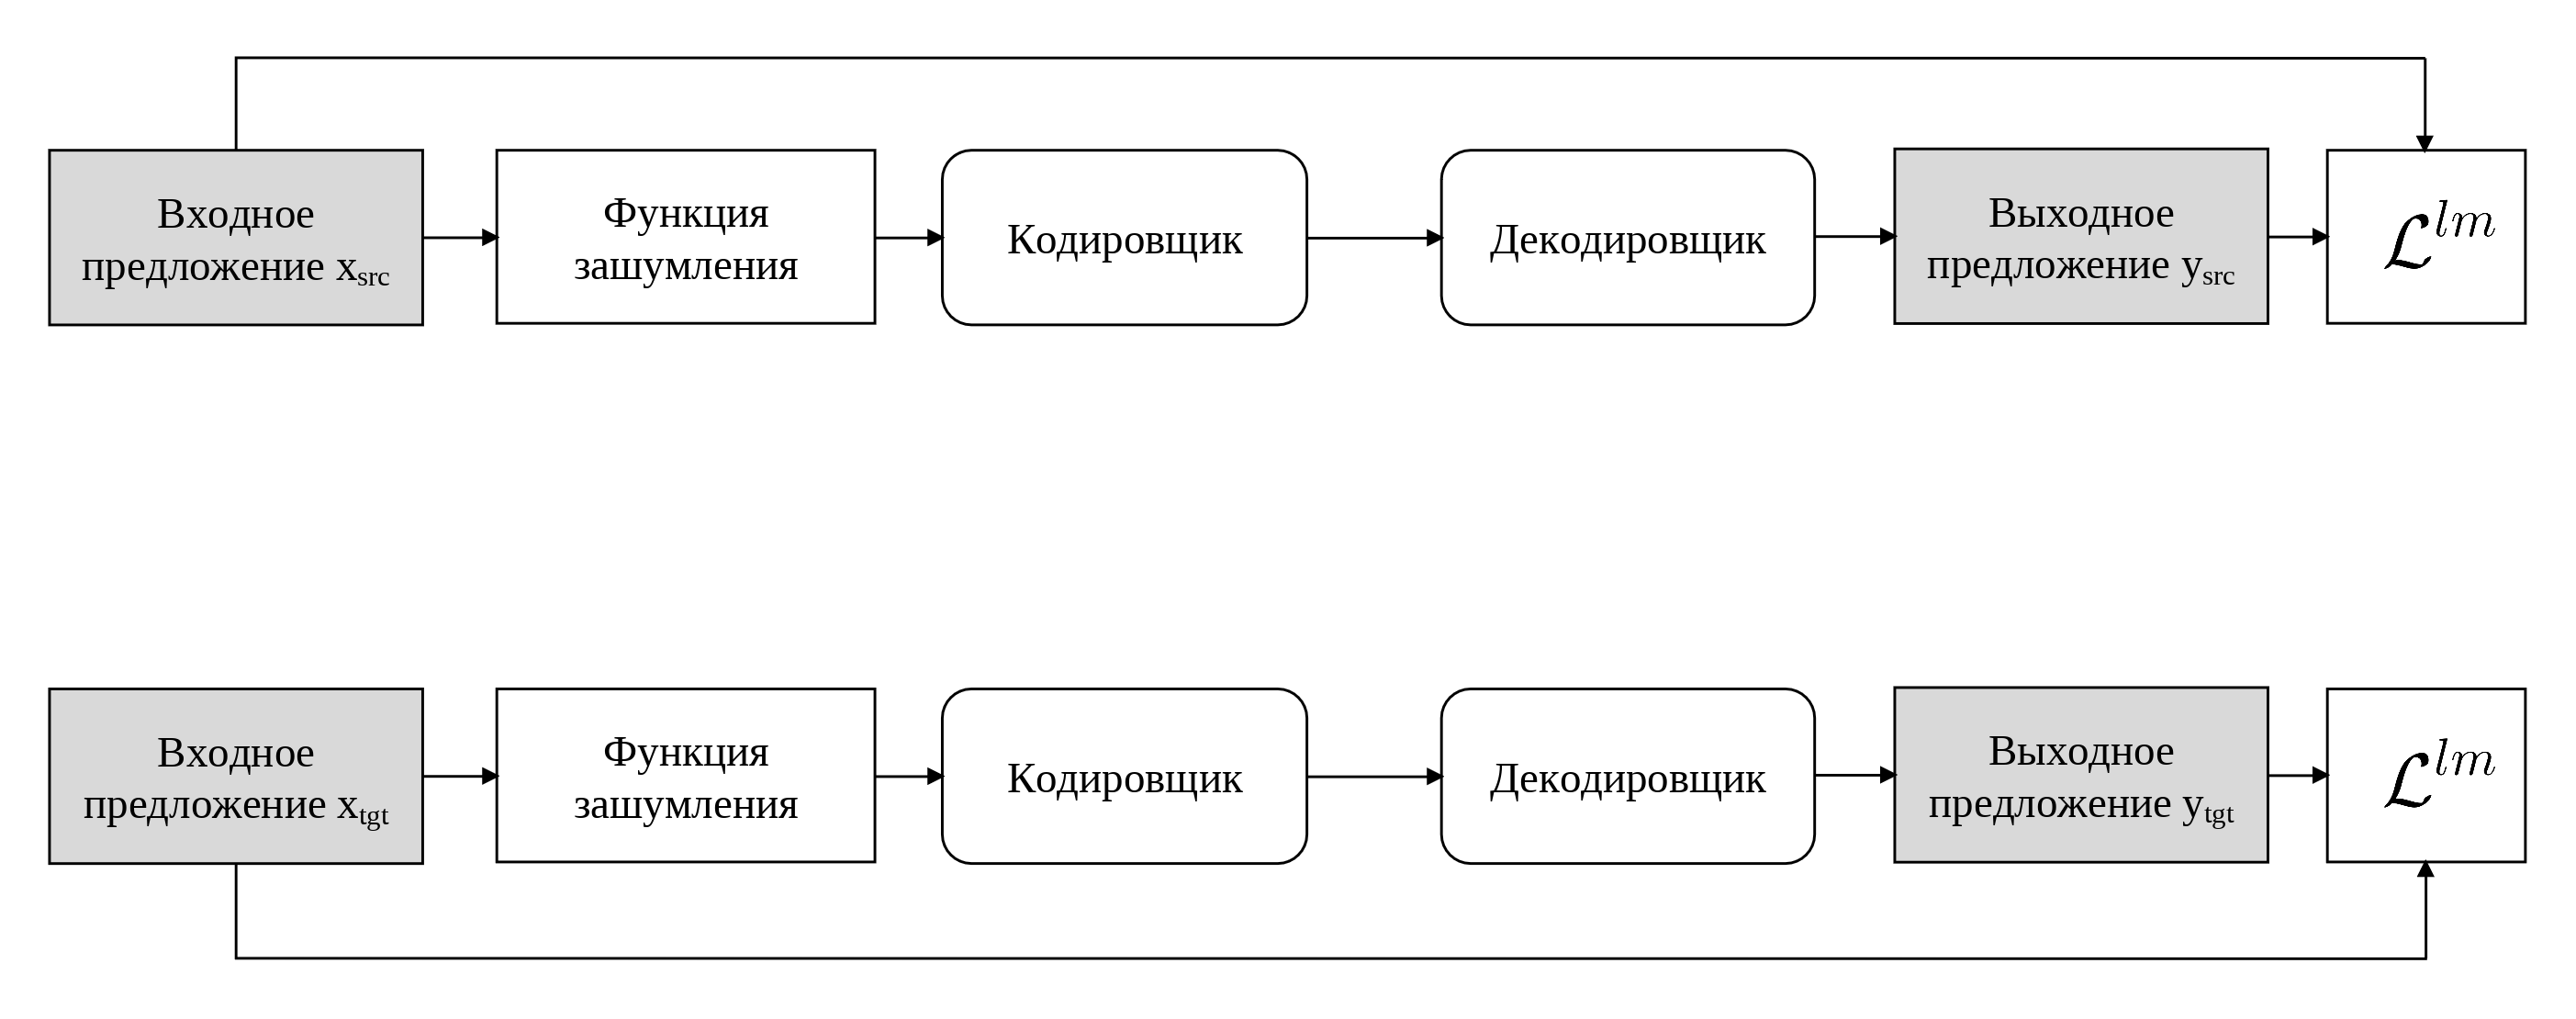
\includegraphics[width=\textwidth]{figures/lample_dae.png}}
  \caption{Обучение denoising auto-encoder}
  \label{fig:lample_dae}
\end{figure}

% Итеративный обратный перевод

% На этом основан механимз back-translation: применим имеющуюся на данную итерацию модель для перевода стиля. Получим парафраз определенного качества. И на полученный парафраз применим обратный перевод: зашумим и пропустим обратно через модель в надежде, что мы сможем восстановить изначальное предложение.

Пространство предложений в исходном и целевом стиле обозначается через $\mathcal{S}$ и $\mathcal{T}$ соответственно, а языковые модели, обученные на исходных и целевых наборах данных, через $P_s$ и $P_t$, соответственно.
Через $P_{s \rightarrow t}$ и $P_{t \rightarrow s}$ обозначим модели парафраза из исходного стиля в целевой и наоборот.
Пусть $u^*(y)$ это предложение в исходном стиле, полученное из $y \in \mathcal{T}$ такое, что $y^*(y) = \arg\max P_{t \rightarrow s}(u|y)$. Подобным образом пусть $v^*(x) = \arg \max P_{s \rightarrow t}(v|x)$.
Таким образом пара $((u^*(y), y)$ и $(x, v^*(x)))$ представляет автоматически перефразированные параллельные предложения, которые могут быть использованы для обучения модели, минимизируя следующую функцию потерь:
$$
\mathcal{L}^{back} = 
\mathbb{E}_{y \sim \mathcal{T}} [-\log P_{s \rightarrow t}(y|u^*(y))] +
\mathbb{E}_{x \sim \mathcal{S}} [-\log P_{t \rightarrow s}(x|v^*(x))]
$$
Этим и выражается третий принцип. Общая схема представленна на рисунке \ref{fig:lample_backtranslation}.

\begin{figure}[ht]
  \centering
  \frame{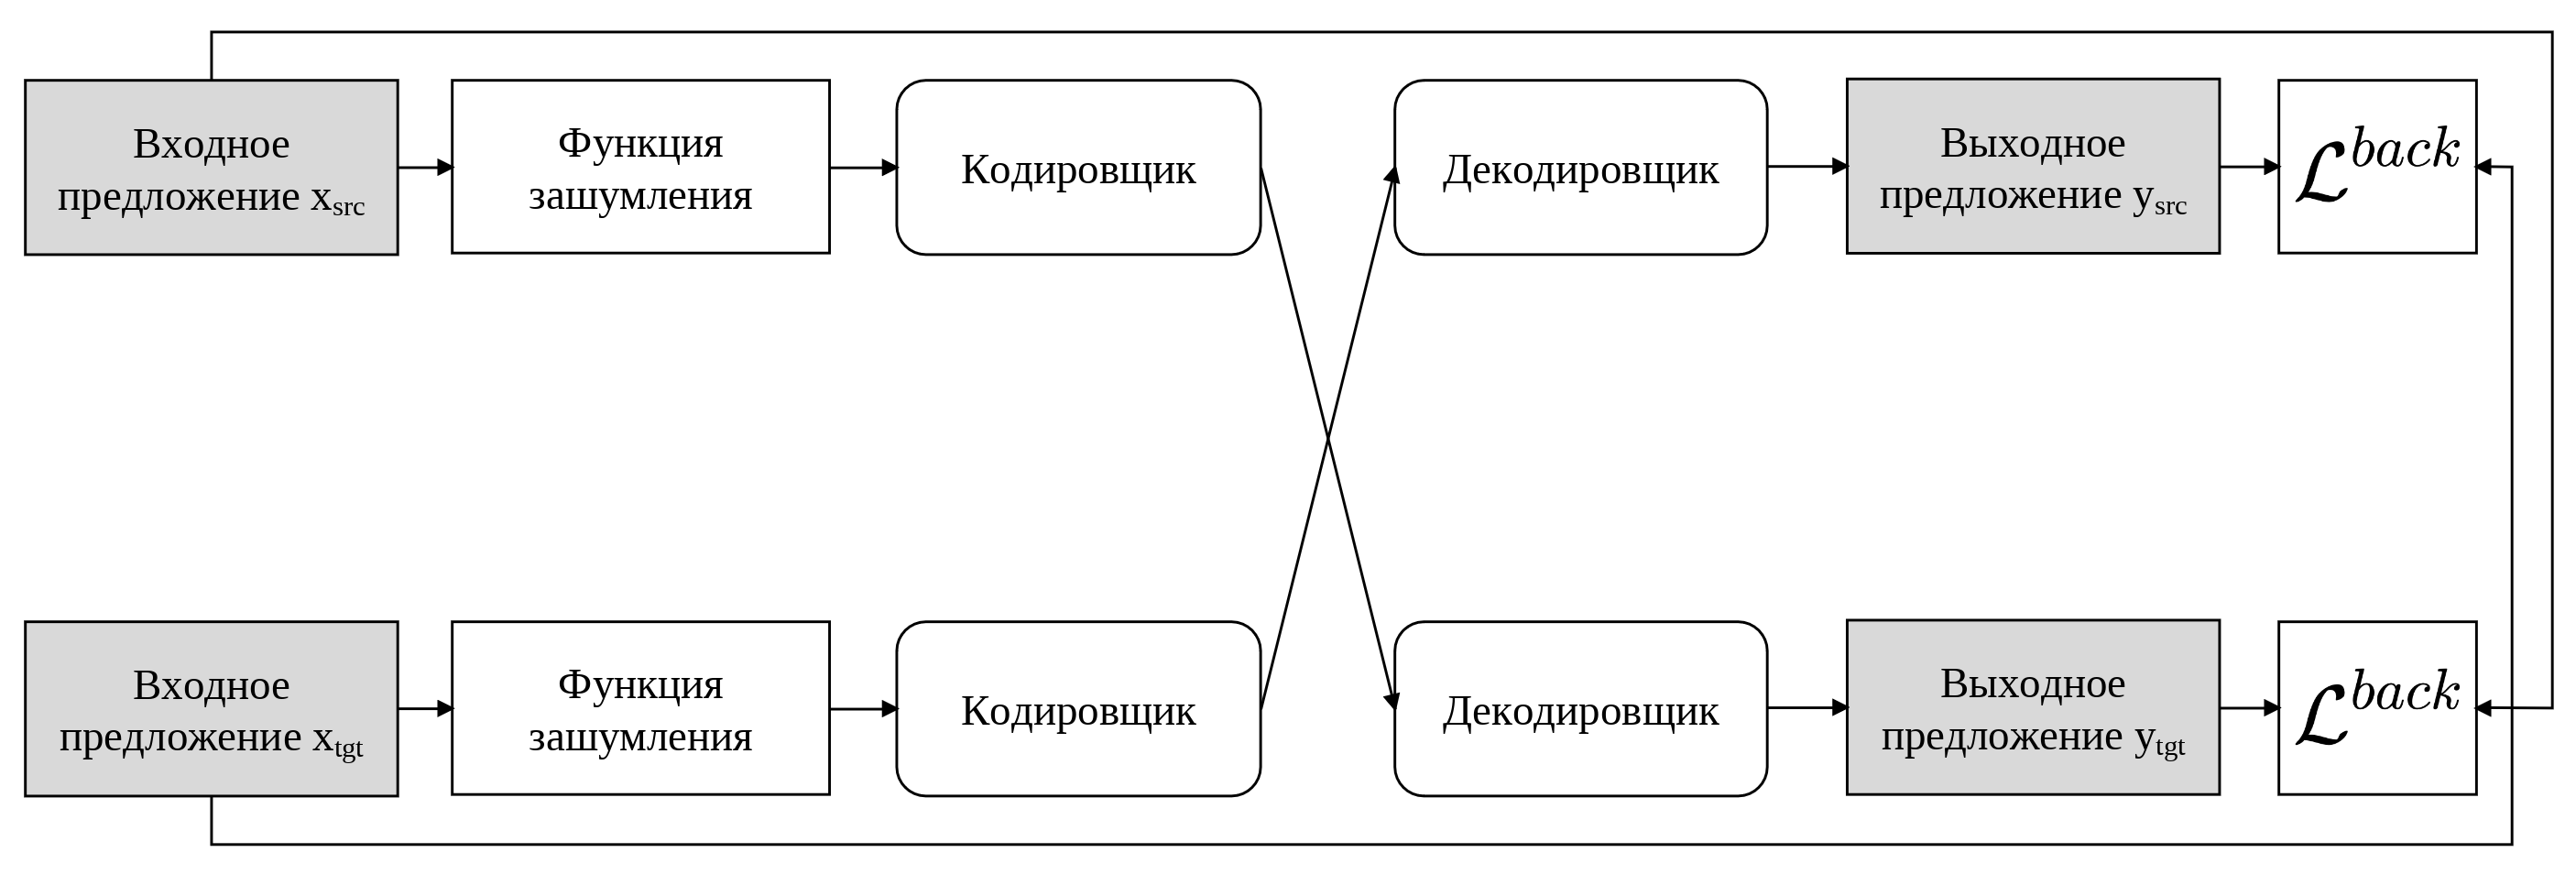
\includegraphics[width=\textwidth]{figures/lample_backtranslation.png}}
  \caption{Обучение с помощью back-translation}
  \label{fig:lample_backtranslation}
\end{figure}

% Он задается 3-мя целевыми функциями:
% \begin{enumerate}
%     \item Это сам авктокодировщик: как хорошо модель может восстановить зашумлённое предложение. Ключевой фактор это функция зашумления, без неё модель будет просто копировать предложения. Здесь эта функция случайным образом удаляла и переставляла местами слова.
%     \item Это функция потерь дискриминатора: дополнительно обучается дискриминатор, который классифицирует исходный стиль эмбеддинга в латентном пространстве. Этот адверсариал-лосс может показаться важным, но на самом деле дальнейшие исследования и мой опыт обучения показывают, что он играет минимальную роль
%     \item И, наконец, третье – самое главное – это кросс-доменная функция потерь. На этом основан механимз back-translation: применим имеющуюся на данную итерацию модель для перевода стиля. Получим парафраз определенного качества. И на полученный парафраз применим обратный перевод: зашумим и пропустим обратно через модель в надежде, что мы сможем восстановить изначальное предложение. Эта кросс-доменная функция потерь измеряет как хорошо это получилось.
% \end{enumerate}

% В качестве модели используется transformer \cite{attention_is_all_you_need}. 
Ключевым параметром является общее использование энкодера между стилями.
Что касается декодера, то авторы заявляют, что его использование оказывает крайне малое влияние \cite{subramanian2019multipleattribute} на качество обучения, однако в рамках данной работы это оказалось ключевым фактором.
Если использовать общий декодер, то модель крайне быстро сходится к тому, что  копирует исходный текст.
Поэтому в итоговой модели используется общий энкодер и два декодера на каждый из стилей.

% Сам процесс обучения итеративный.
% В качестве инициализации используются эмбеддинги fastText и BPE-токенизация. Так как речь идет не о машинном переводе, а о переносе стиля и язык у обоих доменов одинаковый, то эмбединги обучаются совместно. 
% Сначала обучаем определенное количество итераций на задачу денойзинга, получаем первое приближение. Полученную модель копируем и замораживаем и используем для переводов для кросс-доменной функции потерь. После определенного количества итераций, обновляем модель парафраза и повторяем до схождения.

% Во всех методах исследования в качестве монодатасета формального стиля используется случайная подвыборка из википедии по размерам равная имеющемуся монодатасету луркморье




Метрики качества указаны в таблице \ref{table:results}, а примеры генерации в приложении \ref{cha:appendix1}.

\section{Guided Generation}
% Интро
Большие языковые модели (large language models, LLMs), типа GPT \cite{gpt2, gpt3}, способны достаточно хорошо изучить распределение своего обучающего набора данных, чтобы затем генерировать реалистичный текст.
При обучении большой языковой модели используется огромный набор данных, собранный по всему интернету, в котором содержатся тексты различного содержания и различных стилей.
Поэтому имеет смысл пытаться управлять генерацией языковой модели, чтобы результирующий текст имел желательную стилевую окраску.

% Суть
В работах \textit{GeDi: Generative Discriminator Guided
Sequence Generation} \cite{krause2020gedi} и \textit{Text Detoxification using Large Pre-trained Neural Models} \cite{dale2021text} предлагается управлять генерацией текста с помощью другой языковой модели, которая обучена на требуемом домене данных.

Предлагаемая модель GeDi состоит из двух компонент:
генеративная модель на основе GPT-2 и дискриминативная модель, тоже на основе GPT-2, но обученная с дополнительными метками стиля на уровне предложений.
Это заставляет модель дискриминатора выучивать распределения слов, обусловленные конкретным стилем.
На каждом шаге генерации, распределение токенов, полученное из основной модели $P_{LM}$ редактируется с помощью модели дискриминатора $P_D$ и правила Байеса:
$$
P(x_t|x_{<t},c) \propto P_{LM}(x_t|x_{<t})P_D(c|x_t,x_{<t})
$$
где $x_t$ это текущий токен, $x_{<t}$ уже сгенерированный текст, а $c$ это желаемый стилистический атрибут (один из $C$ классов).
Первый член генерируется основной языковой моделью $P_{LM}$, а второй вычисляется с помощью правила Байеса и дополнительной условной языковой модели $P_{CC}$.
Таким образом, токены, которые более вероятно окажутся в тексте желаемым стилем, получают более высокую вероятность:
$$
P_D(c|x_t, x_{<t}) \propto P(c)P_{CC}(x,x_{<t}|c)
$$
Принцип работы проиллюстрирован на рисунке \ref{fig:gedi_original}.
\begin{figure}[ht]
  \centering
  \frame{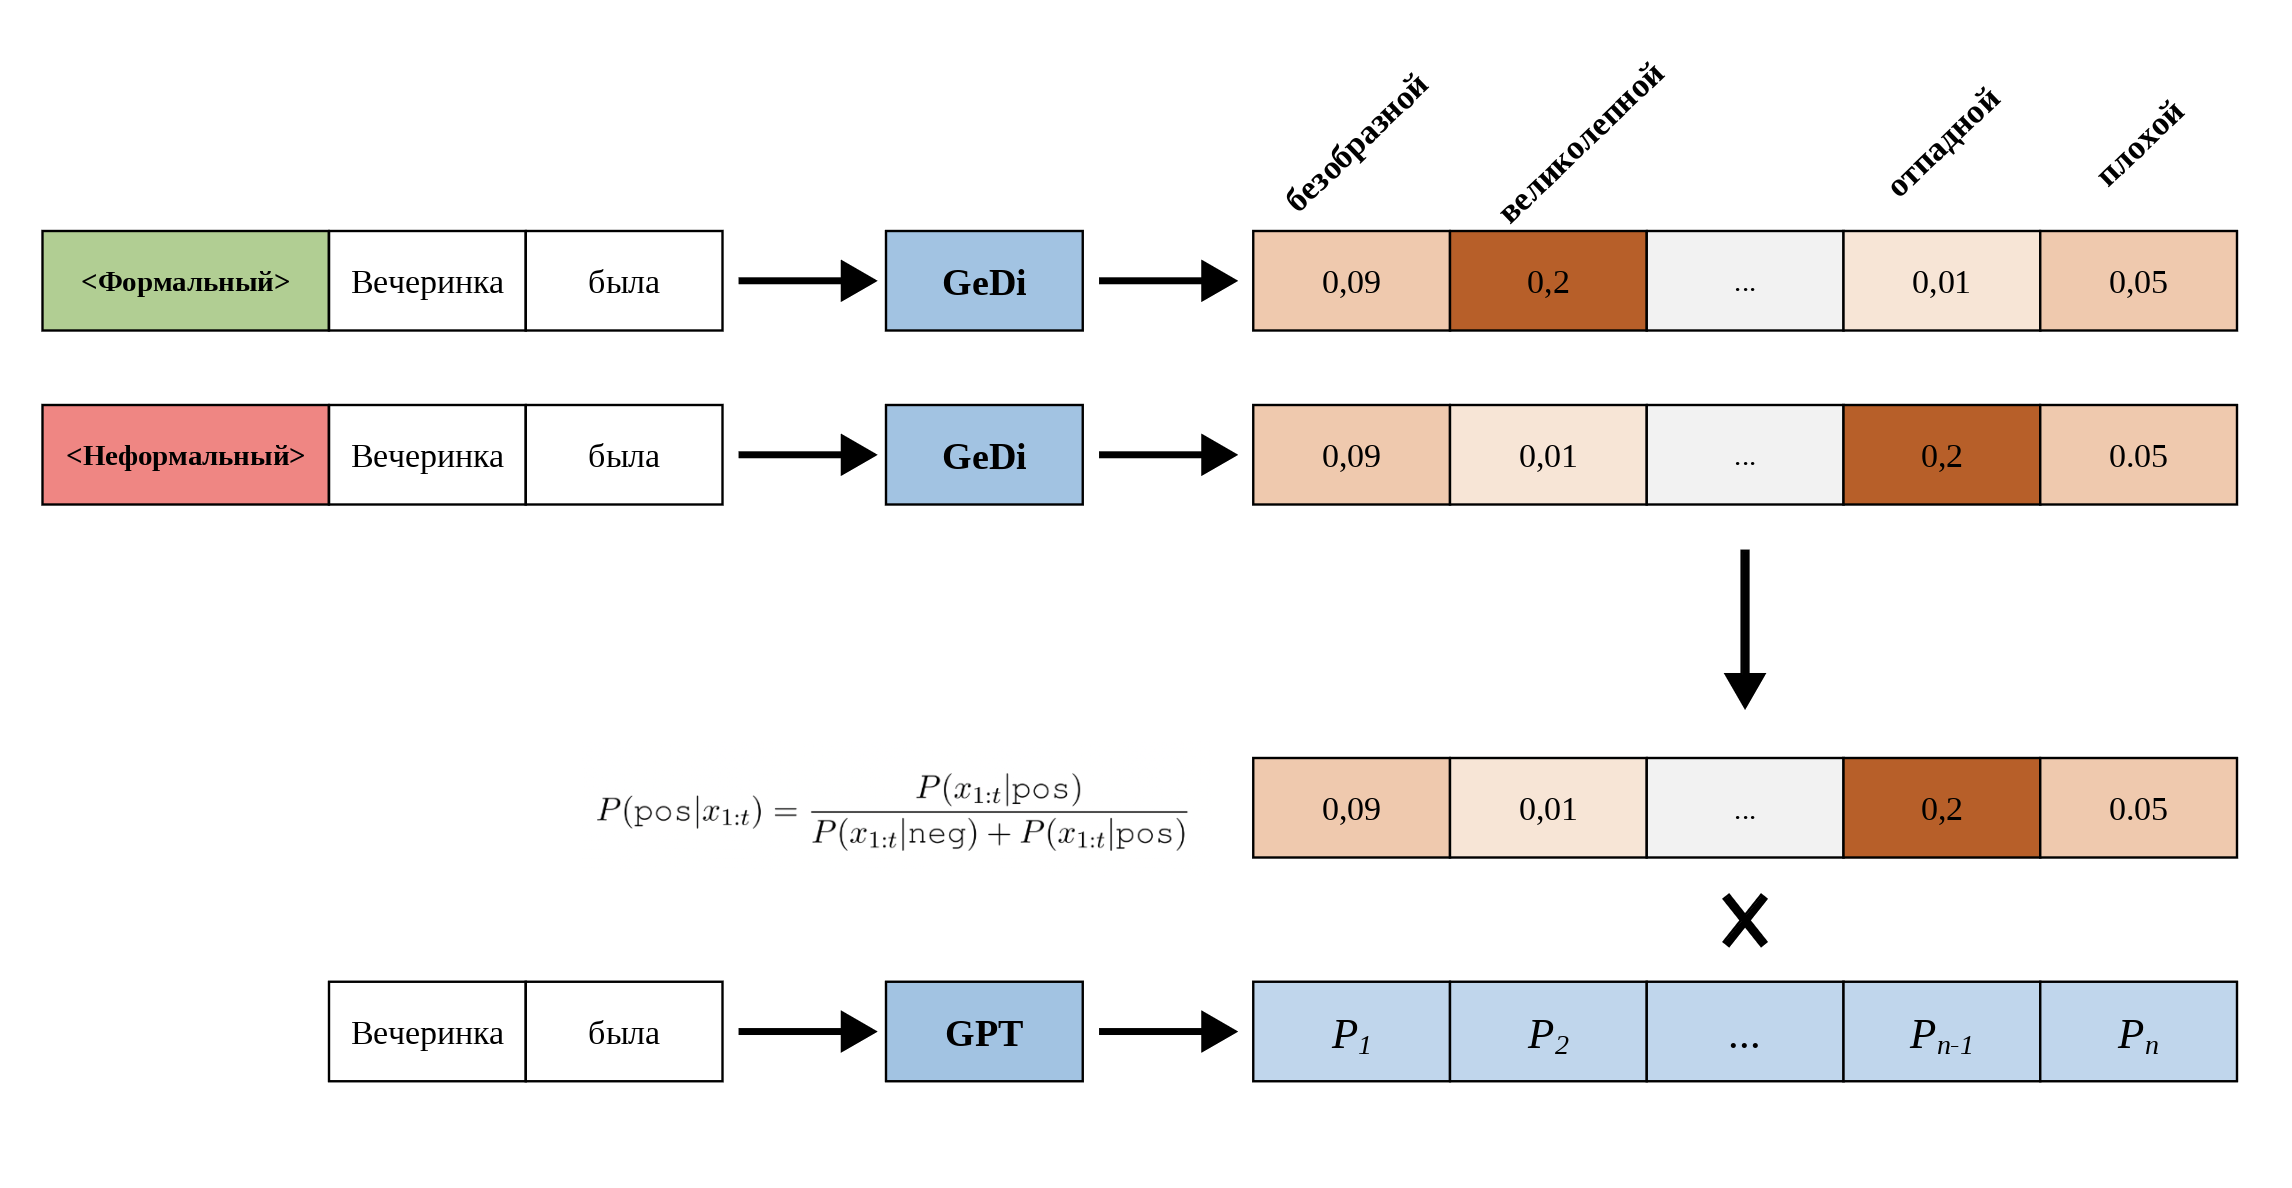
\includegraphics[width=1.0\textwidth]{figures/gedi_original.png}}
  \caption{Модель GeDi}
  \label{fig:gedi_original}
\end{figure}

Чтобы сохранить содержание предложения в работе \cite{dale2021text} предлагается заменить основную языковую модель на модель, обученную на генерацию парафраза.
Пусть $x$ это исходное предложение, $T$ длинна сгенерированного текста $y$, а $c$ это желаемый стиль, то предлагаемая модель моделирует следующую вероятность:
$$
P(y_t|y_{<t},x,x) \propto P_{LM}(y_t|y_{<t}, x)P(c|y_t,y_{<t},x)
\approx P_{LM}(y_t|y_{<t},x)P_D(c|y_t,y_{<t})
$$

Последнее это аппроксимация, потому что вероятность класса должна быть обусловленна как $x$, так и $y$.
Однако это приближение, хотя и не является полностью оправданным, позволяет     отделить модель парафраза (которая требует параллельного корпуса для обучения) от модели стиля (которая требует только текстов с метками стиля, не обязательно параллельных).
Общий принцип работы изображен на рисунке \ref{fig:gedi_paragedi}
\begin{figure}[ht]
  \centering
  \frame{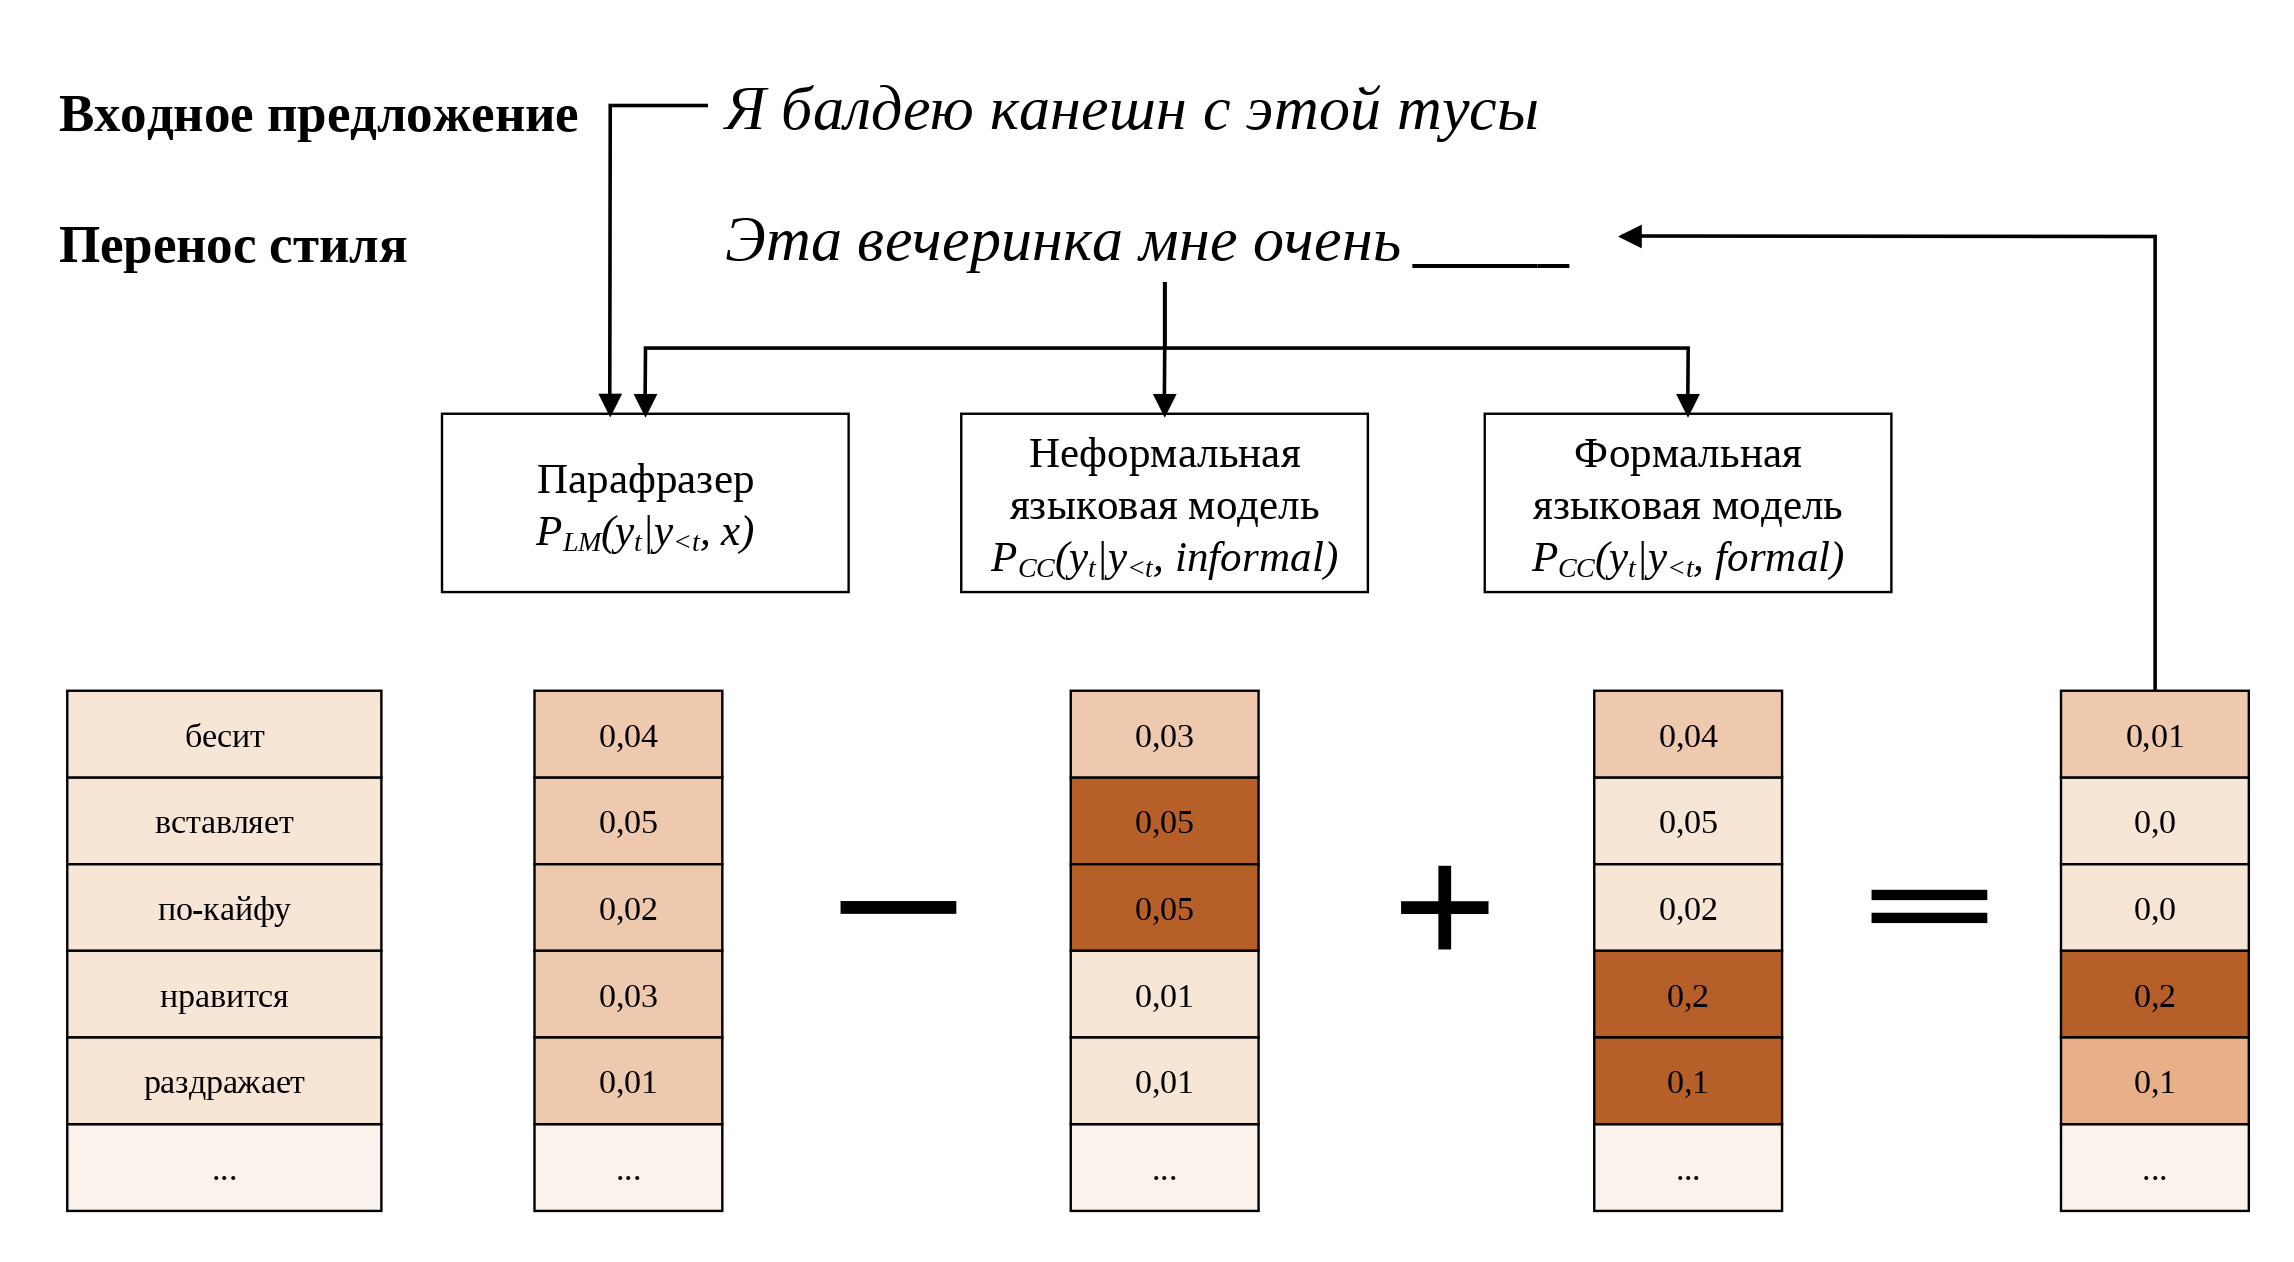
\includegraphics[width=1.0\textwidth]{figures/gedi_detox.png}}
  \caption{Использование модели парафразера в GeDi}
  \label{fig:gedi_paragedi}
\end{figure}

% Обучение
Функция потерь $\mathcal{L}_{ParaGeDi}$ состоит из линейной комбинации двух других функций потерь: генеративной $\mathcal{L}_G$, используемого в обучении языковой модели, и дискриминативной $\mathcal{L}_D$, которая отдаляет разные классы друг от друга в латентном пространстве.
$$
\mathcal{L}_G = - \frac{1}{N} \sum_{i=1}^N 
\frac{1}{T_i} \sum_{t=1}^{T_i} \log P (y_t^{(i)}|y_{<t}^{(i)}, c^{(i)})
$$
$$
\mathcal{L}_D = - \frac{1}{N} \sum_{i=1}^N \log P(c^{(i)}|y_{1:T_i}^{(i)})
$$
$$
\mathcal{L}_{ParaGeDi} = \lambda \mathcal{L}_D + (1 - \lambda) \mathcal{L}_G
$$

В качестве условной языковой модели была использована \texttt{ai-forever/rugpt3large\_based\_on\_gpt2}, а в качестве модели парафраза был взят предобученный \texttt{cointegrated/rut5-base-paraphraser}.

% Результаты и примеры
Метрики качества итогового алгоритма представлены в таблице \ref{table:results}, а примеры генерации в приложении \ref{cha:appendix1}.


% Можно заметить, что задача по переводу из неформального в формальный стиль также оказалась трудновыполнимой, но по сравнению с предыдущим методом был получен прирост в 0,12 по переводу в формальный стиль.

Заметим, что основаные на референсах n-грамные метрики значительно ухудшились, но в то же время можно наблюдать вполне удовлетворительные парафразы.
Здесь стоит сделать вывод и подтвердить другие недавние исследования \cite{li2018delete, mir2019evaluating, shen2022evaluation} о том, что несмотря на наличие параллельного набора данных данные метрики для этой задачи являются не самыми адекватными.
Ведь каждый конкретный стиль может быть выражен разными конструкциями и нет однозначного сопоставления.





\section{Parameter-efficient fine-tuning}
% Общая идея
Параметро-эффективные методы (Parameter-Efficient Fine-Tuning, PEFT) зарекомендовали себя как очень простой и в то же время крайне результативный подход к решению большинства задач.

Общая идея всех методов сводится к:
\begin{enumerate}
    \item использованию больших предобученных языковых моделей (Large Language Models, LLMs);
    \item заморозке всех её параметров;
    \item добавлению небольшого (могут быть десятые доли одного процента от всех параметров) количества дообучаемых параметров;
    \item обучению этих параметров на небольшом наборе данных.
\end{enumerate}

Такой подход даёт следующие преимущества:
\begin{itemize}
    \item если, при наличии набора данных низкого качества, во время классического дообучения (fine-tuning) модель могла ухудшить качество на некоторых задачах, то в этом семействе методов подобного не наблюдается;
    \item значительно снижается необходимое количество размеченных данных – от нескольких сотен до нескольких тысяч примеров;
    \item удобство использования в итоговой системе, потому что достаточно иметь одну большую модель и сколь угодно много адаптеров к ней, которые можно быстро переключать между собой по мере необходимости;
    \item легко дообучать на поступающих новых данных.
\end{itemize}

\subsection{LoRA}
Low-Rank Adaptation of Large Language Models (LoRA) -- метод дообучения, основанный на заморозке весов предобученной модели и добавлении обучаемых матриц ранговой декомпозиции в каждый слой аркитектуры модели, значительно сокращая количество обучаемых параметров \cite{lora}.

Пусть имеется предобученная авторегрессивная языковая модель $P_\Phi(y|x)$, параметризованная $\Phi$.
Каждая задача представлена обучающим набором данных пар контекст-ответ: $\mathcal{Z} = \{(x_i, y_i)\}_{i=1,...,N}$, где оба $x_i$ и $y_i$ представляют собой последовательность токенов.
Во время полноценного дообучения (fine-tuning) модель инициализирована предобученными весами $\Phi_0$ и обновляется как $\Phi_0 + \Delta \Phi$, многократно следуя градиенту для решения максимизационной задачи условного языкового моделирования:
$$
\max_{\Phi}
\sum_{(x,y)\in \mathcal{Z}}
\sum_{t=1}^{|y|}
\log(P_\Phi(y_t|x,y_{<t}))
$$

Основным недостатком является то, что для каждой задачи обучается различный набор параметров $\Delta\Phi$, размерность которого $|\Delta\Phi|$ равна $|\Phi_0|$.
Соответственно, с увеличением размера предобученной модели, хранение и разворачивание множества реплик предобученной модели становится всё более сложной задачей.

В данном подходе применяется более эффективный с точки зрения параметров подход, при котором приращение параметра $\Delta\Phi = \Delta\Phi(\Theta)$ для конкретной задачи дополнительно кодируется набором параметров $\Theta$ гораздо меньшего размера $|\Theta| \ll |\Phi_0|$.
Задача нахождения $\Delta\Phi$ превращается в задачу оптимизации по $\Theta$:
$$
\max_\Theta
\sum_{(x,y)\in \mathcal{Z}}
\sum_{t=1}^{|y|}
\log(p_{\Phi_0 + \Delta\Phi(\Theta)}(y_t|x,y_{<t}))
$$

Нейронная сеть состоит из множества полносвязных слоёв, которые выполняют матричное перемножение.
Матрицы весов в этих слоях обычно являются полноранговыми.
Исследования показывают, что при адаптации к специфической задаче предобученные подели имеют маленькую "`внутреннюю размерность"' и могут эффективно обучаться, несмотря на случайную проекцию в меньшее подпространство \cite{aghajanyan2020intrinsic}.
Из данного наблюдения вытекает гипотеза, что обновления веса моделей тоже имеют небольшую "`внутреннюю размерность"'.
Для предобученной матрицы весов $W_0 \in \mathbb{R}^{d \times k}$ ограничивается её обновления, представляя его в виде разложения низкого ранга $W_0+\Delta W = W_0 + BA$, где $B \in \mathbb{R}^{d \times k}, A\in \mathbb{R}^{r \times k}$ и ранг $r \ll min(d,k)$.
Во время обучения матрица $W_0$ заморожена и не получает обновлений от градиента, в то время как $A$ и $B$ являются обучаемыми параметрами.
Оба $W_0$ и $\Delta W = BA$ умножаются на одинаковый вектор, а их соответствующие выходные вектора по-координатно суммируются.
Для $h = W_0 x$ модифицированный прямой проход:
$$h = W_0x + \Delta W x = W_0x + BAx$$
Данное выражение изображено на рисунке \ref{fig:lora}.
Для $A$ используется случайная Гауссова инициализация, а $B$ инициализируется нулями, так что $\Delta W = BA$ равна нуля в начале обучения.

\begin{figure}[ht]
  \centering
  \frame{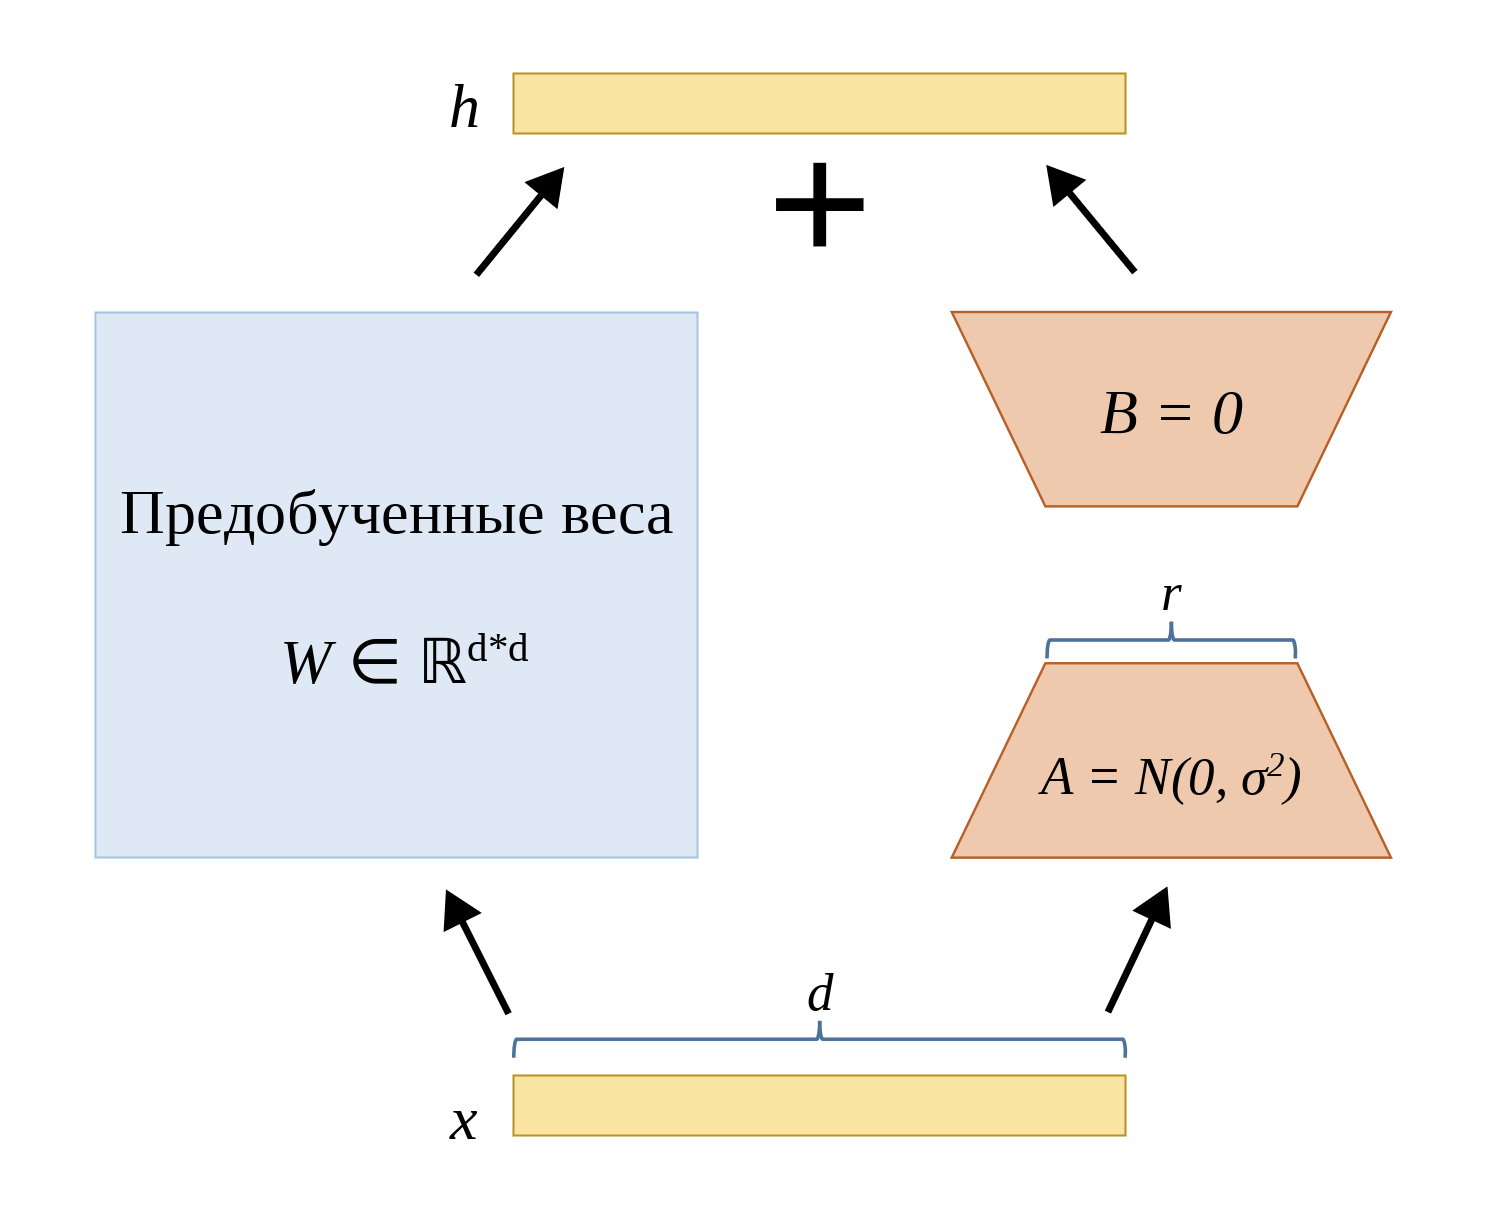
\includegraphics[width=0.7\textwidth]{figures/lora.png}}
  \caption{Параметризация весов в алгоритме LoRA. Обновляются только матрицы $A$ и $B$}
  \label{fig:lora}
\end{figure}

В работе с помощью данного алгоритма была дообучена модель \texttt{cointegrated/rut5-base-paraphraser} на собранном наборе данных.
Метрики качества указаны в таблице \ref{table:results}, а примеры генерации в  в приложении \ref{cha:appendix1}.


\subsection{P-Tuning}
Данный метод основан на автоматическом поиске затравок (prompts) в непрерывном пространства \cite{gpt_understands_too}.

Пусть дана предобученная языковая модель $\mathcal{M}$.
Последовательность дискретных входных токенов 
$x_{1:n} = \{x_0, x_1, ..., x_n\}$
будет сопоставлена с входными эмбеддингами 
$\{\mathbf{e}(x_o), \mathbf{e}(x_1), ..., \mathbf{e}(x_n)\}$
с помощью предварительно обученного слоя ембеддингов
$\mathbf{e} \in \mathcal{M}$.
В конкретном случае, зависящем от контекста $\mathbf{x}$, часто используются выходные эмбеддинги набора целевых токенов  $\mathbf{y}$ для последующей обработки.

Функция затравки (промпта) $\mathbf{p}$ - организовать контекст $\mathbf{x}$, результат $\mathbf{y}$ и саму себя в шаблон $T$.
Для задачи переноса стиля текста шаблоном может быть "<Перепиши предложение "`$\mathbf{x}$"' в неформальном стиле: "`$\mathbf{y}$"'">.
Здесь "<Перепиши предложение ... в неформальном стиле: ..."> это затравка, $\mathbf{x}$ это контекст, а $\mathbf{y}$ это результат.

Пусть $\mathcal{V}$ это словарный запас языковой модели $\mathcal{M}$, а $[P_i]$ является $i$-ым токеном шаблона $T$.

Имея шаблон $T = \{ [P_{0:i}],x,[P_{i+1:m}], y \}$, дискретная затравка удовлетворяет условию $[P_i] \in \mathcal{V}$ и превращает $T$ в
$$\{ \mathbf{e}([P_{0:i}]), \mathbf{e}(\mathbf{x}), \mathbf{e}([P_{i+1:m}]),\mathbf{e}(\mathbf{y}) \}$$

В отличии от этого, P-tuning воспринимает $[P_i]$ как псевдо-токены и превращает шаблон в
$$\{h_0, ..., h_i, \mathbf{e}(\mathbf{x}), h_{i_1}, ..., h_m, \mathbf{e}(\mathbf{x})\}$$
где $h_i(0 \leqslant i < m)$ это обучаемые эмбеддинги.
Это позволяет находить лучшие непрерывные затравки вне словарного запаса, которым оперирует языковая модель.
Сравнение дискретного поиска и P-tuning приллюстрировано на рисунке \ref{fig:p_tuning}.

Имея функцию потерь $\mathcal{L}$ можно дифференциально оптимизировать непрерывные затравки $h_i(0 \leqslant i < m)$ как
$$\hat{h}_{0:m} = \arg\min_h \mathcal{L} (\mathcal{M}(\mathbf{x},\mathbf{y}))$$

\begin{figure}[ht]
  \centering
  \frame{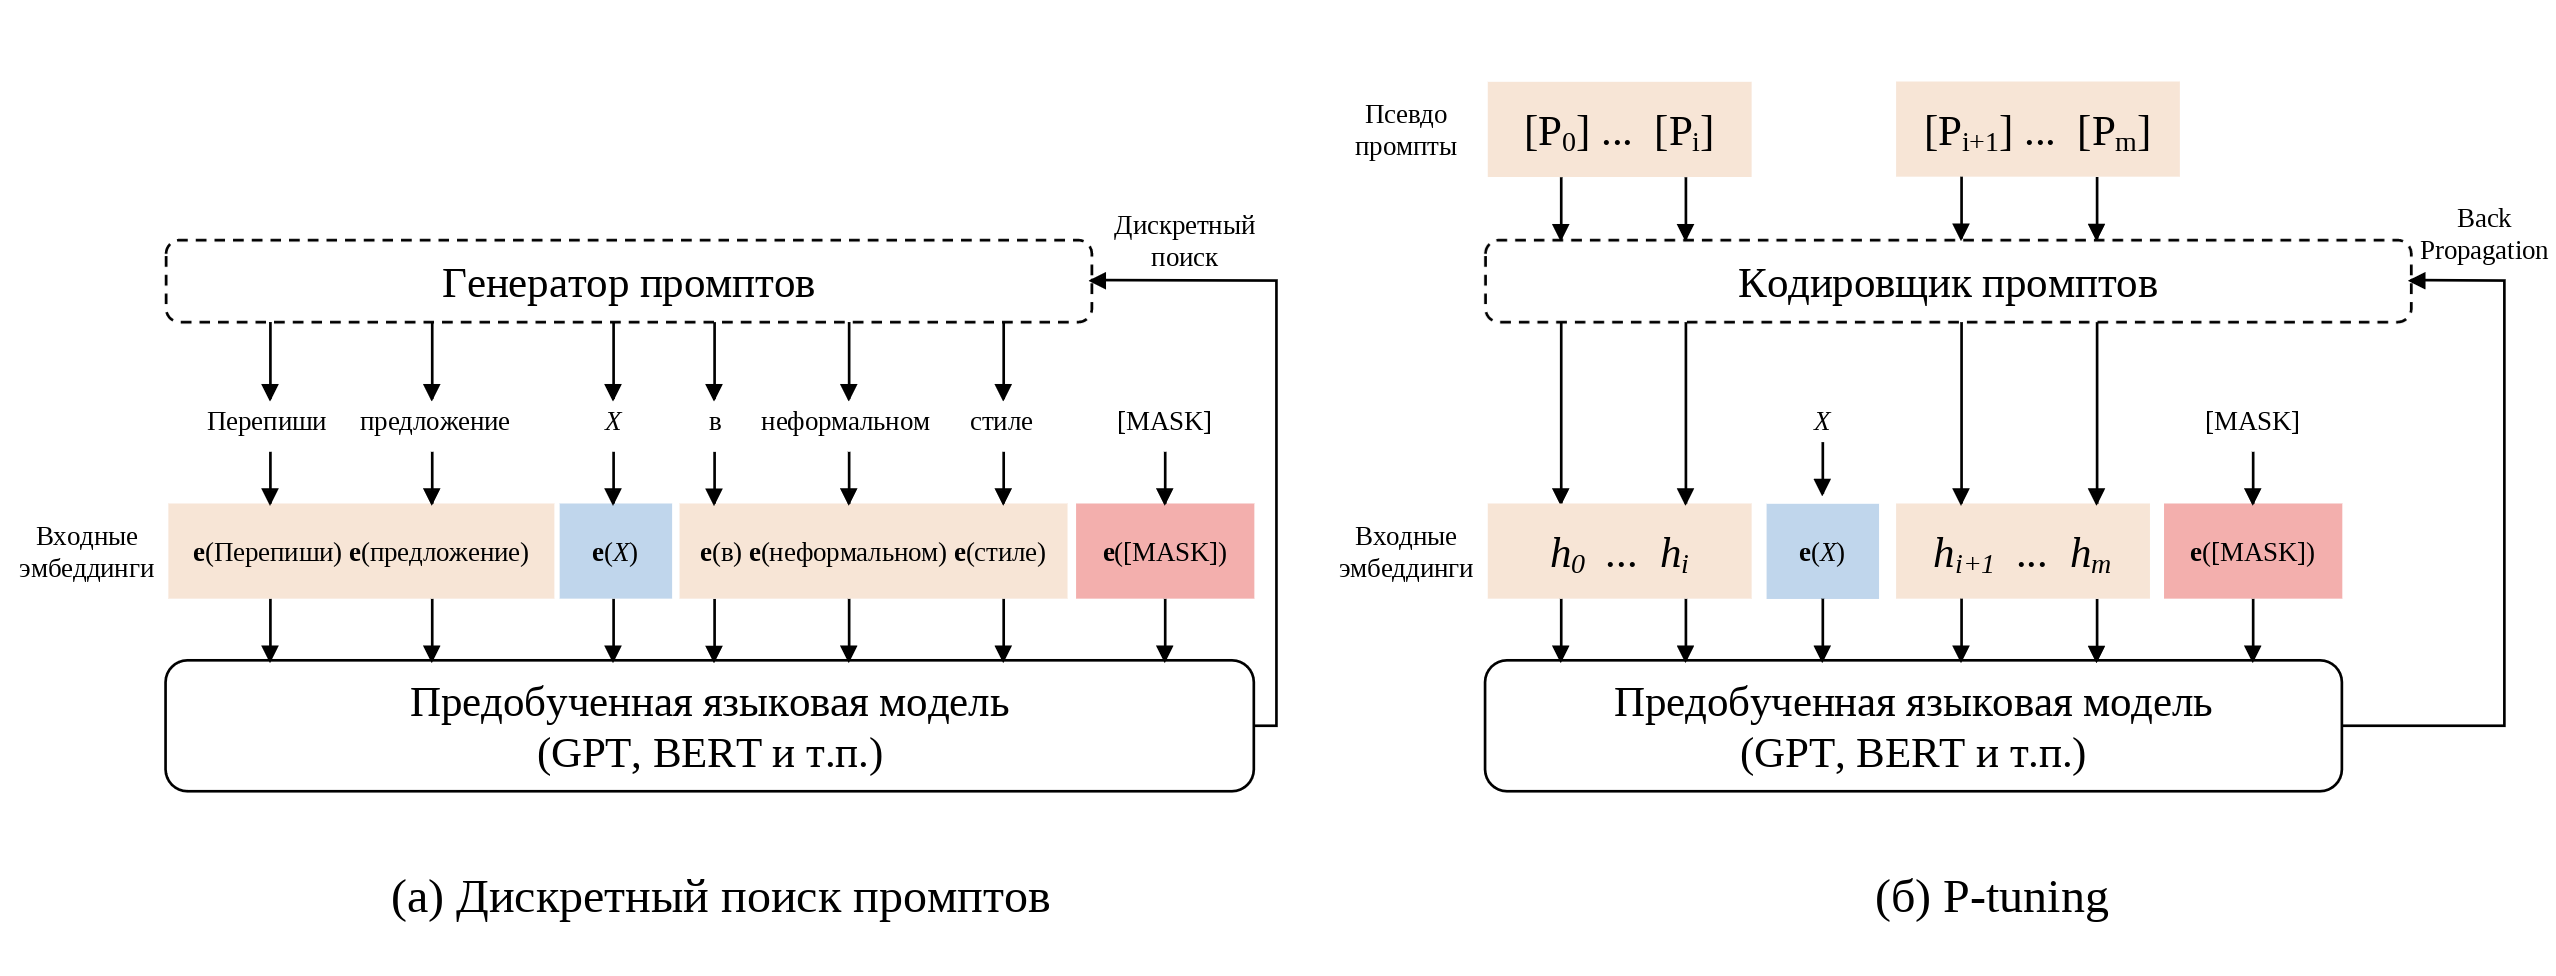
\includegraphics[width=1.0\textwidth]{figures/p_tuning.png}}
  \caption{P-tuning}
  \label{fig:p_tuning}
\end{figure}

В работе с помощью данного алгоритма была дообучена модель \texttt{ai-forever/rugpt3small\_based\_on\_gpt2} на собранном наборе данных.
Метрики качества указаны в таблице \ref{table:results}, а примеры генерации в  в приложении \ref{cha:appendix1}.

\section{Few-Shot LLM}
Появление таких больших генеративных языковых моделей, как ChatGPT и GPT-4 \cite{gpt3, openai2023gpt4} показало, что после превышения определённого числа параметров модель становится достаточно большой, чтобы решать большинство задач во few-shot или даже zero-shot режиме.

В данной работе так же был исследован вопрос, как хорошо справится подобная модель с задачей переноса стиля текста.
Для этого была выбрана модель GPT-4 от OpenAI.
Была подобрана затравка с несколькими примерами изменения формальности текста и модели было дано задание по этому подобию изменить формальность других предложений.
Пример затравки и генераций представлен в приложении \ref{cha:appendix1}.
Можно сделать вывод, что GPT-4 полностью справился с поставленной ему задачей.


\section{Результаты}
Результаты метрик по всем проведенным экспериментам представлены в таблице \ref{table:results}, а примеры генераций в приложении \ref{cha:appendix1}.

Можно сделать вывод, что лучше всего показали себя большие языковые модели, способные без какого-либо дообучения на конкретную задачу показывать результат лучше, чем целенаправленно обученные на задачу модели.
Языковые модели прошлого поколения (GPT-3, T-5 и пр.) с помощью параметро-эффективных методов обучения могут показать хороший результат, особенно в случае отсутствия большого набора данных.
Более старые алгоритмы показывают качество генераций намного хуже.

Обучение без учителя и Guided Generation показали лучшие метрики SacreBLEU и METEOR.
Использование предобученных языковых моделей в сочетании с параметро-эффективными методами дообучения и использование собранного параллельного набора данных дало наилучший результат с точки зрения комбинации метрик Style Score и Semantic Score.
Это подтверждает другие исследования \cite{li2018delete, mir2019evaluating}, что использование метрик, основанных на n-граммах и сравнении с референсами, зачастую не даёт адекватной оценки качества алгоритма.

\begin{table}[ht]
\small
\centering
\caption{Метрики качества исследованных подходов}
\label{table:results}
\begin{tabular}{|p{0.35\textwidth}|c|c|c|c|}
\hline
% \multicolumn{4}{c}{wiki --> lurk / lurk --> wiki}
% Метод & SacreBLEU & METEOR & StyleScore & SemanticScore   \\ \hline \hline
\multirow{2}{*}{Метод} & SacreBLEU & METEOR & StyleScore & SemanticScore   \\ \cline{2-5}
 & \multicolumn{4}{c|}{wiki $\rightarrow$ lurk / lurk $\rightarrow$ wiki} \\ \hline \hline
Unsupervised DAE & 40,5/38,8 & 0,6/0,59 & 0,22/0,6 & 0,82/0,78 \\\hline
Guided Generation & 12,7/6,7 & 0,35/0,27 & 0,13/0,72 & 0,81/0,75 \\\hline
LoRA(ruT5-paraphraser) & 3,04/3,35 & 0,25/0,26 & 0,3/0,75 & 0,79/0,8 \\\hline
P-Tuning (GPT) & 3,16/4,56 & 0,23/0,23 & 0,56/0,92 & 0,73/0,78 \\\hline
\end{tabular}
\end{table}

Также обратим внимание, что с точки зрения StyleScore задача трансфера стиля из формального вики в неформальный лурк является намного более сложной задачей, с которой во всех рассмотренных методах наблюдаются трудности.
Как было упомянуто в параграфе \ref{cha:analysis:sec:datasets} перефразирование в неформальный стиль является более трудной задачей даже для человека.
Стилистическая специфика лурка более сложна и модели труднее её выучить, нежели формальный стиль Википедии.


% \begin{equation}
%     \frac{i + s + d}{n},
%     \label{lev_eq}
% \end{equation}
% \par где $i$ -- количество вставок;
% \par $s$ -- количество замен;
% \par $d$ -- количество удалённых символов;
% \par $n$ -- количество символов/слов в целевой последовательности.
